\definecolor{c231f20}{RGB}{35,31,32}

\def \globalscale {1.000000}
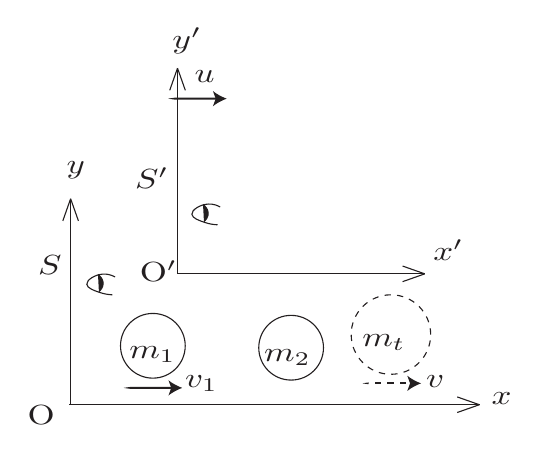
\begin{tikzpicture}[y=1cm, x=1cm, yscale=\globalscale,xscale=\globalscale, every node/.append style={scale=\globalscale}, inner sep=0pt, outer sep=0pt]
  \path[draw=c231f20,miter limit=10.0] (1.9029, -0.417) -- (1.9029, -3.029);



  \node[text=c231f20,cm={ 1.26,-0.0,-0.0,1.0,(0.4958, -1.8209)},anchor=south west] (text9035) at (0.0, 0.0){$y$};



  \path[draw=c231f20,miter limit=10.0] (1.9029, -0.417) -- (1.8039, -0.6982);



  \path[draw=c231f20,miter limit=10.0] (1.9029, -0.417) -- (2.0021, -0.6982);



  \path[draw=c231f20,miter limit=10.0] (5.043, -3.029) -- (1.9029, -3.029);



  \path[draw=c231f20,miter limit=10.0] (5.043, -3.029) -- (4.7614, -2.93);



  \path[draw=c231f20,miter limit=10.0] (5.043, -3.029) -- (4.7614, -3.1282);



  \node[text=c231f20,cm={ 1.26,-0.0,-0.0,1.0,(5.8931, -4.6911)},anchor=south west] (text5310) at (0.0, 0.0){$x$};



  \path[draw=c231f20,miter limit=10.0] (0.5453, -2.0749) -- (0.5453, -4.6871);



  \node[text=c231f20,cm={ 1.29,-0.0,-0.0,1.0,(1.8391, -0.2352)},anchor=south west] (text733) at (0.0, 0.0){$y^\prime$};



  \node[text=c231f20,cm={ 1.26,-0.0,-0.0,1.0,(1.365, -1.9444)},anchor=south west] (text7650) at (0.0, 0.0){$S^\prime$};



  \path[draw=c231f20,miter limit=10.0] (0.5453, -2.0749) -- (0.4464, -2.3561);



  \path[draw=c231f20,miter limit=10.0] (0.5453, -2.0749) -- (0.6445, -2.3561);



  \path[draw=c231f20,miter limit=10.0] (5.742, -4.6911) -- (0.5265, -4.6911);



  \path[draw=c231f20,miter limit=10.0] (5.7364, -4.6911) -- (5.4552, -4.5921);



  \path[draw=c231f20,miter limit=10.0] (5.7364, -4.6911) -- (5.4552, -4.79);



  \node[text=c231f20,cm={ 1.26,-0.0,-0.0,1.0,(5.1525, -2.8623)},anchor=south west] (text4647) at (0.0, 0.0){$x^\prime$};



  \node[text=c231f20,cm={ 1.26,-0.0,-0.0,1.0,(0.1341, -3.0361)},anchor=south west] (text989) at (0.0, 0.0){$S$};



  \node[text=c231f20,cm={ 1.26,-0.0,-0.0,1.0,(0.0, -4.9427)},anchor=south west] (text5260) at (0.0, 0.0){O};



  \path[fill=c231f20] (1.7822, -0.8041).. controls (1.8082, -0.7996) and (1.8341, -0.7967) .. (1.86, -0.793).. controls (1.8664, -0.7922) and (1.873, -0.7908) .. (1.8793, -0.7906).. controls (1.8857, -0.7906) and (1.8923, -0.7911) .. (1.8987, -0.7908) -- (2.4037, -0.7908) -- (2.4037, -0.8173) -- (1.8987, -0.8173).. controls (1.8923, -0.8173) and (1.8857, -0.8173) .. (1.8793, -0.8176).. controls (1.873, -0.8173) and (1.8664, -0.816) .. (1.86, -0.8152).. controls (1.8341, -0.8115) and (1.8082, -0.8086) .. (1.7822, -0.8041) -- cycle;



  \path[fill=c231f20] (2.527, -0.8041).. controls (2.4691, -0.8255) and (2.3974, -0.8623) .. (2.3529, -0.9009) -- (2.3879, -0.8041) -- (2.3529, -0.7072).. controls (2.3974, -0.7461) and (2.4691, -0.7826) .. (2.527, -0.8041) -- cycle;



  \node[text=c231f20,cm={ 1.26,-0.0,-0.0,1.0,(2.119, -0.6038)},anchor=south west] (text256) at (0.0, 0.0){$u$};



  \node[text=c231f20,cm={ 1.26,-0.0,-0.0,1.0,(1.4258, -3.1231)},anchor=south west] (text8061) at (0.0, 0.0){O$^\prime$};



  \path[draw=c231f20,miter limit=10.0] (1.5899, -3.9426) circle (0.4109cm);



  \path[draw=c231f20,miter limit=10.0] (3.3457, -3.9672) circle (0.4109cm);



  \path[fill=c231f20] (1.2176, -4.4773).. controls (1.2435, -4.4728) and (1.2695, -4.4699) .. (1.2954, -4.4662).. controls (1.3018, -4.4654) and (1.3084, -4.4641) .. (1.3147, -4.4638).. controls (1.3211, -4.4638) and (1.3277, -4.4643) .. (1.334, -4.4641) -- (1.8391, -4.4641) -- (1.8391, -4.4905) -- (1.334, -4.4905).. controls (1.3277, -4.4905) and (1.3211, -4.4905) .. (1.3147, -4.4908).. controls (1.3084, -4.4905) and (1.3017, -4.4892) .. (1.2954, -4.4884).. controls (1.2695, -4.4847) and (1.2435, -4.4818) .. (1.2176, -4.4773) -- cycle;



  \path[fill=c231f20] (1.9624, -4.4773).. controls (1.9045, -4.4987) and (1.8328, -4.5355) .. (1.7883, -4.5741) -- (1.8232, -4.4773) -- (1.7883, -4.3804).. controls (1.8328, -4.4193) and (1.9045, -4.4558) .. (1.9624, -4.4773) -- cycle;



  \node[text=c231f20,cm={ 1.26,-0.0,-0.0,1.0,(2.001, -4.5268)},anchor=south west] (text588) at (0.0, 0.0){$v_1$};



  \path[draw=c231f20,miter limit=10.0] (1.1102, -3.0689).. controls (1.0814, -3.0528) and (1.0268, -3.0279) .. (0.9583, -3.0319).. controls (0.8559, -3.0377) and (0.7461, -3.1059) .. (0.7509, -3.162).. controls (0.7551, -3.2112) and (0.8464, -3.2422) .. (0.9131, -3.265).. controls (0.9776, -3.2869) and (1.0351, -3.2935) .. (1.0766, -3.2954);



  \path[draw=c231f20,fill=c231f20,miter limit=10.0] (0.893, -3.0361).. controls (0.9136, -3.0528) and (0.9514, -3.088) .. (0.9578, -3.1366).. controls (0.9655, -3.1951) and (0.9237, -3.2385) .. (0.9046, -3.2557);



  \path[draw=c231f20,miter limit=10.0] (2.4445, -2.1796).. controls (2.4156, -2.1635) and (2.3611, -2.1386) .. (2.2926, -2.1426).. controls (2.1902, -2.1484) and (2.0804, -2.2167) .. (2.0852, -2.2728).. controls (2.0894, -2.322) and (2.1807, -2.3529) .. (2.2474, -2.3757).. controls (2.3119, -2.3977) and (2.3693, -2.4043) .. (2.4109, -2.4061);



  \path[draw=c231f20,fill=c231f20,miter limit=10.0] (2.227, -2.1468).. controls (2.2476, -2.1635) and (2.2855, -2.1987) .. (2.2918, -2.2474).. controls (2.2995, -2.3058) and (2.2577, -2.3492) .. (2.2386, -2.3664);



  \path[draw=c231f20,miter limit=10.0,dash pattern=on 0.0794cm] (4.6133, -3.7999) circle (0.5048cm);



  \path[fill=c231f20] (4.2508, -4.4196).. controls (4.2773, -4.4151) and (4.3037, -4.4119) .. (4.3302, -4.4082) -- (4.3302, -4.431).. controls (4.3037, -4.4273) and (4.2773, -4.4241) .. (4.2508, -4.4196) -- cycle;



  \path[fill=c231f20] (4.4095, -4.4064) rectangle (4.4889, -4.4328);



  \path[fill=c231f20] (4.5683, -4.4064) rectangle (4.6477, -4.4328);



  \path[fill=c231f20] (4.727, -4.4064) rectangle (4.8064, -4.4328);



  \path[fill=c231f20] (4.9953, -4.4196).. controls (4.9374, -4.441) and (4.8657, -4.4778) .. (4.8212, -4.5164) -- (4.8562, -4.4196) -- (4.8212, -4.3228).. controls (4.8657, -4.3617) and (4.9374, -4.3982) .. (4.9953, -4.4196) -- cycle;



  \node[text=c231f20,cm={ 1.26,-0.0,-0.0,1.0,(5.0604, -4.4773)},anchor=south west] (text3774) at (0.0, 0.0){$v$};



  \node[text=c231f20,cm={ 1.26,-0.0,-0.0,1.0,(1.2907, -4.151)},anchor=south west] (text6657) at (0.0, 0.0){$m_1$};



  \node[text=c231f20,cm={ 1.26,-0.0,-0.0,1.0,(3.0044, -4.1974)},anchor=south west] (text5195) at (0.0, 0.0){$m_2$};



  \node[text=c231f20,cm={ 1.26,-0.0,-0.0,1.0,(4.2508, -4.0)},anchor=south west] (text5524) at (0.0, 0.0){$m_t$};


\end{tikzpicture}

